% Drawing 154/07-13 -- folder 154, batch 07, archive page 136 (PDF page 137).
% Transcription: dessins en couleur : en haut, un grand fuseau entre deux croisements orange, bordé d'un arc orange, traversé de droites vert clair, la droite vert foncé et deux chemins en tirets bruns qui passent par les sommets ; à gauche, un petit repère fléché ($\omega$, $\varpi$). À droite, un cercle au crayon traversé de deux paires de droites orange, une droite vert clair et une vert foncé fléchée, les sommets $s_4$, $t_3$ (chiffres entourés), les étiquettes $D_1 = D_{19}$, $D_{18}$, $D_4$, et au croisement de droite « $5 = 19$ ! ». Au milieu, un croisement orange sur une droite verte avec des flèches $\varpi$, $\omega$ ; à gauche en bas, un croisement enjambé d'une courbe au crayon, avec la légende « \uncertain{non sans triangle} ». En bas, un grand fuseau entre deux croisements orange, bordé d'un arc orange, les sommets marqués $s_1$, $s_2$, $s_3$, $s_4$, $s_5$, $s_6 = s_1$, $t_2$, $t_3$, avec des numéros bleus et noirs $1$ à $19$ autour des sommets ; à droite, une ellipse au crayon traversée de croisements orange et de la droite vert foncé
% Kind: large spindles between two orange crossings crossed by light green lines, with brown dashed paths; small frames and disks; the sequence D_1 ... D_20. Method 2 (schematic redraw from the facsimile). Status: partial.
% Notes: Colour drawings over a printed program listing (« PROGRAM CRAY7 ... BONJOUR », 19 Aug 82; not reproduced), read from the page view. Top: a large spindle between two orange crossings, bordered by an orange arc, crossed by light green lines, the dark green line and two brown dashed paths through the vertices. Left, a small arrowed frame (omega) and crossings on a light green line. Right, a disk with light and dark green lines crossing orange lines, labels D_1 = D_19, D_18, s, t (only D_1 = D_19 placed). Bottom: the same spindle in a second state, crossed by orange crossings, with the vertex labels; below it the sequence « s_1 s_2 ... ; D_1 D_2 ... D_20 = D_5 » given as one label; small spindles with crossings left and right. Strands schematic. Still differs from the facsimile: BONJOUR », 19 Aug 82; not reproduced), read from the page view. Strands schematic.
% Coordinates: 1 unit = 1 mm = 1/100 of the crop width (bbox in page fractions: [0.166, 0.146, 0.964, 0.528]).
% Redrawn by Claude (claude-opus-5-5), issue #73, 2026-11-07; not checked by a human; not compiled (no TeX in the session).
% Revised by Claude (claude-opus-5-5) 2026-11-09 (issue #128) after Michel's check: vertices snapped to exact intersections (drawn points on their lines, meeting ends on the stroke they meet, near-concurrent lines through one computed point, curve ends on their rim); labels at \small as in folder 80 batch 3. Status: partial.
% Rights: reproduces part of the work -- behind RENDER_TRANSCRIPTS, never published by itself.
\documentclass[tikz,border=3pt]{standalone}
\usepackage{amsmath,amssymb}
\usetikzlibrary{patterns,arrows.meta}
\tikzset{Or/.style={orange!90!black}, Ye/.style={yellow!80!orange}, Lg/.style={green!60!black!70}, Dg/.style={green!45!black}, Br/.style={brown!80!black}, Rd/.style={red!85!black}, Bl/.style={blue!70!black}, Gy/.style={black!40}, pencil/.style={black!45}, struck/.style={black!35}, mark/.style={circle,draw,inner sep=1.3pt}, pt/.style={circle,fill,inner sep=0.9pt}, opt/.style={circle,draw,fill=white,inner sep=1.1pt}}
\begin{document}
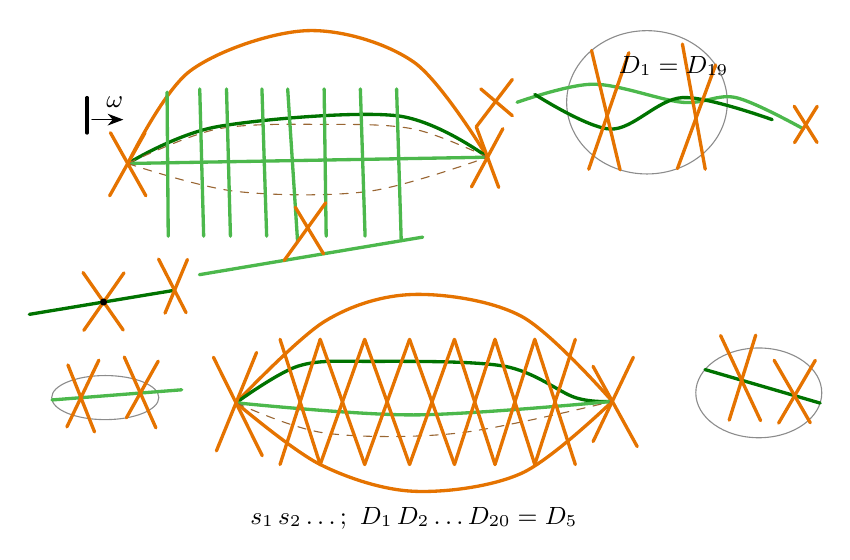
\begin{tikzpicture}[x=1mm,y=1mm,line cap=round,line join=round,font=\scriptsize]
\draw[Or,very thick] plot[smooth, tension=0.55] coordinates {(11.36,-19.17) (19.3,-7.4) (34.1,-2.3) (47.7,-6.3) (57.05,-18.37)};
\draw[Dg,very thick] plot[smooth, tension=0.55] coordinates {(11.36,-19.17) (22.7,-14.5) (45.5,-13.1) (57.05,-18.37)};
\draw[Lg,very thick] (11.36,-19.17) -- (57.05,-18.37);
\draw[Br,dashed] plot[smooth, tension=0.55] coordinates {(11.36,-19.17) (22.7,-14.8) (36.4,-14.2) (47.7,-14.8) (57.05,-18.37)};
\draw[Br,dashed] plot[smooth, tension=0.55] coordinates {(11.36,-19.17) (25,-22.7) (42,-22.7) (57.05,-18.37)};
\draw[Lg,very thick] (16.35,-10.11) -- (16.5,-28.4);
\draw[Lg,very thick] (20.5,-9.7) -- (21,-28.4);
\draw[Lg,very thick] (23.9,-9.7) -- (24.4,-28.4);
\draw[Lg,very thick] (28.4,-9.7) -- (29,-28.4);
\draw[Lg,very thick] (31.67,-9.71) -- (32.93,-29.11);
\draw[Lg,very thick] (36.3,-9.7) -- (36.56,-28.41);
\draw[Lg,very thick] (40.9,-9.7) -- (41.5,-28.4);
\draw[Lg,very thick] (45.5,-9.7) -- (46.09,-28.98);
\draw[Or,very thick] (9.16,-15.26) -- (13.66,-23.27);
\draw[Or,very thick] (13.55,-15.27) -- (9.06,-23.27);
\draw[Or,very thick] (55.62,-14.51) -- (58.47,-22.21);
\draw[Or,very thick] (59,-14.75) -- (55.01,-22.15);
\draw[very thick] (6.2,-10.8) -- (6.2,-15.3);
\draw[-{Stealth[length=2mm]}] (6.8,-13.6) -- (10.8,-13.6);
\node[inner sep=1pt] at (9.7,-11.4) {\small $\omega$};
\draw[Lg,very thick] (20.46,-33.29) -- (48.82,-28.52);
\draw[Or,very thick] (32.65,-24.74) -- (36.22,-30.64);
\draw[Or,very thick] (36.5,-24.16) -- (31.23,-31.48);
\draw[Dg,very thick] (-1.14,-38.33) -- (17.31,-35.27);
\draw[Or,very thick] (5.68,-33.02) -- (10.78,-40.32);
\draw[Or,very thick] (10.88,-33.06) -- (5.78,-40.36);
\node[pt] at (8.29,-36.76) {};
\draw[Or,very thick] (15.27,-31.31) -- (18.77,-38.12);
\draw[Or,very thick] (18.94,-31.36) -- (16.09,-38.18);
\draw[pencil] (77.3,-11.4) ellipse[x radius=10.2, y radius=9.1];
\draw[Lg,very thick] plot[smooth, tension=0.55] coordinates {(60.8,-11.4) (70.5,-9.1) (81.8,-11.4) (88.6,-10.8) (97.14,-14.76)};
\draw[Dg,very thick] plot[smooth, tension=0.55] coordinates {(63.06,-10.4) (72.7,-14.8) (81.8,-10.8) (93.2,-13.6)};
\draw[Or,very thick] (70.26,-4.82) -- (73.88,-19.97);
\draw[Or,very thick] (75,-5.1) -- (69.9,-19.9);
\draw[Or,very thick] (81.8,-4) -- (84.7,-19.9);
\draw[Or,very thick] (86.01,-6.66) -- (81.17,-19.82);
\draw[Or,very thick] (56.2,-9.7) -- (60.2,-13.1);
\draw[Or,very thick] (60.2,-8.5) -- (55.62,-14.51);
\draw[Or,very thick] (96,-11.9) -- (98.9,-16.5);
\draw[Or,very thick] (98.92,-11.91) -- (96.04,-16.52);
\node[inner sep=1pt] at (80.7,-6.8) {\small $D_1=D_{19}$};
\draw[Or,very thick] plot[smooth, tension=0.55] coordinates {(25.11,-49.56) (36.4,-39.2) (47.7,-35.8) (61.4,-38.6) (72.9,-49.38)};
\draw[Or,very thick] plot[smooth, tension=0.55] coordinates {(25.11,-49.56) (35.8,-57.4) (47.7,-60.8) (61.4,-58.5) (72.9,-49.38)};
\draw[Dg,very thick] plot[smooth, tension=0.55] coordinates {(25.11,-49.56) (33,-44.9) (42,-44.3) (59.1,-44.9) (68.2,-48.9) (72.9,-49.38)};
\draw[Lg,very thick] plot[smooth, tension=0.55] coordinates {(25.11,-49.56) (47.7,-51.1) (72.9,-49.38)};
\draw[Br,dashed] plot[smooth, tension=0.55] coordinates {(25.11,-49.56) (36.4,-53.4) (53.4,-53.4) (72.9,-49.38)};
\draw[Or,very thick] (30.7,-41.5) -- (35.8,-57.4);
\draw[Or,very thick] (35.8,-41.5) -- (30.7,-57.4);
\draw[Or,very thick] (35.8,-41.5) -- (41.45,-57.4);
\draw[Or,very thick] (41.45,-41.5) -- (35.8,-57.4);
\draw[Or,very thick] (41.45,-41.5) -- (47.15,-57.4);
\draw[Or,very thick] (47.15,-41.5) -- (41.45,-57.4);
\draw[Or,very thick] (47.15,-41.5) -- (52.85,-57.4);
\draw[Or,very thick] (52.85,-41.5) -- (47.15,-57.4);
\draw[Or,very thick] (52.85,-41.5) -- (58,-57.4);
\draw[Or,very thick] (58,-41.5) -- (52.85,-57.4);
\draw[Or,very thick] (58,-41.5) -- (63.05,-57.4);
\draw[Or,very thick] (63.05,-41.5) -- (58,-57.4);
\draw[Or,very thick] (63.05,-41.5) -- (68.2,-57.4);
\draw[Or,very thick] (68.2,-41.5) -- (63.05,-57.4);
\draw[Or,very thick] (22.24,-43.78) -- (28.44,-56.28);
\draw[Or,very thick] (27.72,-43.17) -- (22.62,-55.67);
\draw[Or,very thick] (70.45,-44.93) -- (76.06,-55.12);
\draw[Or,very thick] (75.57,-43.78) -- (70.46,-54.48);
\draw[pencil] (8.5,-48.9) ellipse[x radius=6.8, y radius=2.8];
\draw[Lg,very thick] (1.74,-49.2) -- (18.21,-47.91);
\draw[Or,very thick] (3.76,-44.76) -- (7.14,-53.26);
\draw[Or,very thick] (7.69,-44.15) -- (3.63,-52.62);
\draw[Or,very thick] (10.92,-43.75) -- (14.93,-52.74);
\draw[Or,very thick] (15.23,-44.27) -- (11.19,-51.47);
\draw[pencil] (91.5,-48.3) ellipse[x radius=8, y radius=5.7];
\draw[Dg,very thick] (84.67,-45.34) -- (99.29,-49.6);
\draw[Or,very thick] (86.65,-41.02) -- (91.73,-51.83);
\draw[Or,very thick] (91.11,-40.97) -- (87.74,-51.77);
\draw[Or,very thick] (93.45,-44.16) -- (98.04,-52.1);
\draw[Or,very thick] (98.68,-44.17) -- (94.02,-52.14);
\node[inner sep=1pt] at (47.7,-64.2) {\small $s_1\,s_2\ldots;\ D_1\,D_2\ldots D_{20}=D_5$};
\end{tikzpicture}
\end{document}
